%-------------------------------------
% This template comes from Anish Athalye (Unofficial University of Cambridge Poster Template). 

% The Poster Template has been modified by Dr. Rahul Raoniar to fulfill B.Tech/Master/Ph.D./PostDoc student's poster presentation requirements.

% Description: I made this unofficial Poster Template for the Indian Institute of Technology Bombay (IITB). Feel free to use it, modify it, and share it. 

% Thank you note: A huge thanks goes to Anish Athalye for the original template.
%-------------------------------------


\documentclass[final]{beamer}

% ====================
% Packages
% ====================
\usepackage{url}
\usepackage[T1]{fontenc}
\usepackage{lmodern}
\usepackage[orientation=portrait,size=a0,scale=1.0]{beamerposter}
\usetheme{gemini}
\usecolortheme{UBI}
\usepackage{graphicx}
\usepackage{booktabs}
\usepackage{tikz}
\usepackage[portuguese]{babel}
\usepackage{pgfplots}
\usepackage{subfigure}
\pgfplotsset{compat=1.14}
\usepackage{anyfontsize}
\usepackage{xcolor}
\usepackage[skip=2pt,font=normalsize]{subcaption}
\usepackage{adjustbox}

% ----------------------------------
% For plotting study methodology
% ----------------------------------

\usepackage{tikz}
\usetikzlibrary{shapes.geometric, arrows}

% Defining Tickz Style
\tikzstyle{startstop} = [rectangle, rounded corners, minimum width=3cm, minimum height=1cm, text centered, text width = 10cm, draw=black, fill=white]

% \tikzstyle{io} = [trapezium, trapezium left angle=70, trapezium right angle=110, minimum width=3cm, minimum height=1cm, text centered, text width = 4.5cm, draw=black, fill=blue!30]

\tikzstyle{process} = [rectangle, minimum width=3cm, minimum height=1cm, text centered, text width = 6cm, draw=black, fill=white, text width = 10cm]

% \tikzstyle{decision} = [diamond, minimum width=3cm, minimum height=1cm, text centered, draw=black, fill=green!30]

\tikzstyle{arrow} = [ultra thick,->,>=stealth]


% ====================
% Lengths
% ====================

% If you have N columns, choose \sepwidth and \colwidth such that
% (N+1)*\sepwidth + N*\colwidth = \paperwidth
\newlength{\sepwidth}
\newlength{\colwidth}
\setlength{\sepwidth}{0.025\paperwidth}
\setlength{\colwidth}{0.45\paperwidth}

\newcommand{\separatorcolumn}{\begin{column}{\sepwidth}\end{column}}

% ====================
% Title
% ====================

\title{Queda de uma mola ideal suspensa com massas distribuídas regularmente}

\author{José Amoreira \inst{1,2} \and João Santos \inst{1} \and João Esteves \inst{1}}

\institute[]{\inst{1}Universidade da Beira Interior \samelineand \inst{2} Centro de Matemática e Aplicações}

% ====================
% Footer (optional)
% ====================

\footercontent{
  Física 2024 \hfill
  UBI - Departamento de Física}
% (can be left out to remove footer)


% ====================
% Logo (optional)
% ====================

% use this to include logos on the left and/or right side of the header:
\logoright{
\includegraphics[scale=1.5]{logos/DF2.png}}
\logoleft{
\includegraphics[scale=1.5]{logos/DF2.png}}

% ====================
% Body
% ====================

\begin{document}

\begin{frame}[t]
\begin{columns}[t]
\separatorcolumn

\begin{column}{\colwidth}

% ----------------------------------
% Abstract
% ----------------------------------
  \begin{block}{Motivação}
    O movimento de queda ilustrado é interessante
    porque parece acontecer que a extremidade inferior da mola como que fica em repouso enquanto a outra cai aceleradamente na direção da primeira. Naturalmente, isto deve-se ao facto de a extremidade inferior da mola se encontrar inicialmente em equilíbrio sob a ação do seu peso e da força elástica nela exercida. A variação da elongação da mola após o início do movimento começa por fazer sentir na extremidade superior, onde a resultante das forças aplicadas (peso e força elástica) tem maior intensidade; na extremidade inferior a situação de equilíbrio estático inicial permanece, até ser atingida pela onda longitudinal de compressão iniciada na extremidade superior.
    Esta explicação qualitativa é convincente mas considera uma mola real, com uma dada distribuição de massa e de elasticidade ao longo do seu comprimento; em suma, uma mola com dinâmica. Ora, nos problemas de física elementar, considera-se desprezável a massa das molas. Assim, as molas aparecem apenas como veículos das interações entre os corpos presos nas suas extremidades; afetam a dinâmica desses corpos mas não têm dinâmica própria. Com este trabalho
    pretendemos verificar, analítica e experimentalmente, se a queda de molas ideais exibe também o efeito referido.
    Uma vez que uma mola ideal não tem massa, não tem dinâmica. Não fica suspensa por uma extremidade, nem cai quando essa extremidade é solta. Devemos pois acrescentar ao problema massas dispostas ao longo da mola (no mínimo dos mínimos, uma massa em cada extremidade), que sentem o efeito das forças (gravítica e elástica) exercidas no sistema e que manifestam o comportamento dinâmico que elas determinam.
  \end{block}
  
% ----------------------------------
% Section: Literature review
% ----------------------------------
  \begin{alertblock}{Resumo}

    jmfjd fgghjgfh

    \heading{Research gaps}
    Pjdnvfj

  \end{alertblock}

\begin{block}{Descrição analítica}
    Aplicando a segunda lei de Newton a este formalismo, ficamos com:
    \begin{align*}
        \ddot x_0 &=-Ng+\omega^2(x_1-x_0)\\[1cm] 
        \ddot x_i &= \omega^2(x_{i-1}-2x_i+x_{i+1}),\qquad i=1, \ldots, N-2\\[1cm]
         \ddot x_{N-1} &=\omega^2(x_{N-2}-x_{N-1})
    \end{align*}    
\end{block}

\begin{block}{Procedimento experimental}
   No começo, observamos a queda do conjunto mola e bola para compreender o seu comportamento. O experimento foi inicialmente realizado com duas bolas e uma mola. Em seguida, repetimos o procedimento com três bolas, dividindo a mola ao meio. Ambas as execuções foram gravadas em câmara lenta, a uma taxa de 120 frames por segundo, e posteriormente analisadas usando o software Tracker.
    \begin{figure}[h]
    \centering
    \includegraphics[width=0.3\textwidth,scale=.5]{images/mola.pdf}
    \caption{Procedimento realizado para 2 e 3 bolas}
    \label{fig:figure2}
\end{figure}
    Em seguida, a constante elástica tanto para a mola completa quanto para a metade da mola foi determinada por meio de outro experimento. Com esses resultados em mãos, os valores teóricos foram calculados utilizando o Python e comparados com os resultados experimentais obtidos pelo Tracker. \emph{(mais informação no código QR)}
\end{block}

% -------------------------------
% Section: Descriptive Statistics
% -------------------------------


\end{column}

\separatorcolumn

\begin{column}{\colwidth}

% -------------------------------
% Section: Results and discussion
% -------------------------------

\begin{block}{Resultados}
    
    Após realizar o procedimento todo explicado no bloco anterior, comparámos então os resultados:
    \begin{figure}
    \centering
    \subfigure[]{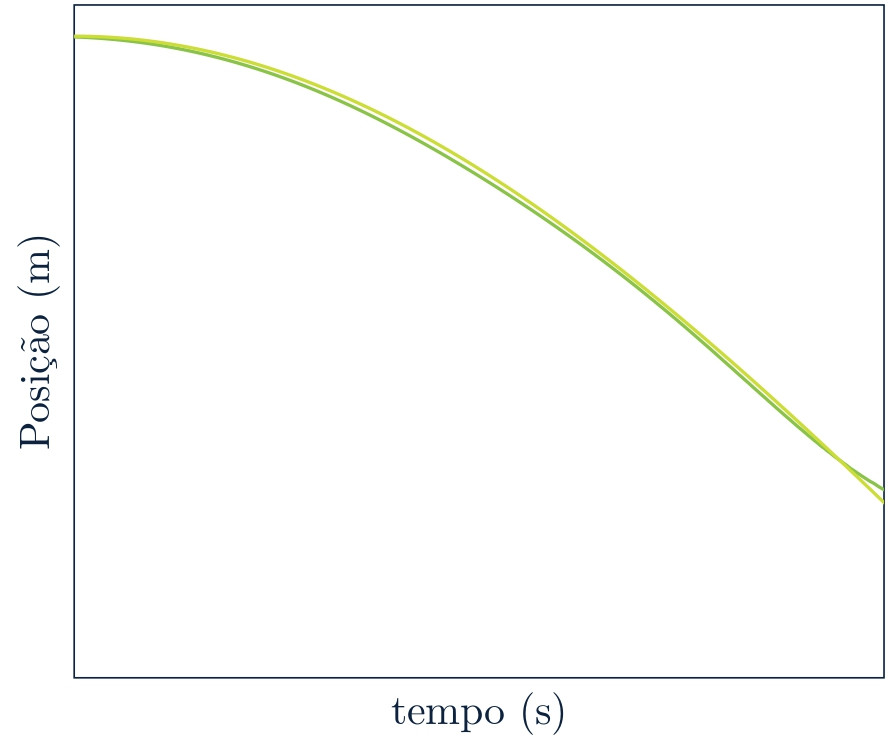
\includegraphics[width=0.3\columnwidth]{images/1.jpg}} 
    \subfigure[]{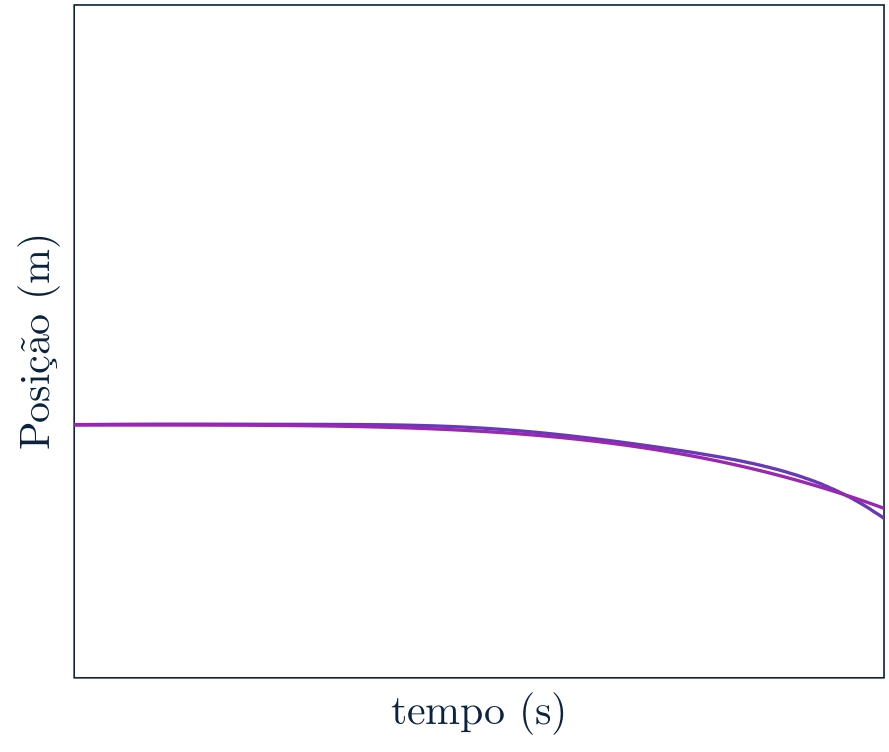
\includegraphics[width=0.3\columnwidth]{images/2.jpg}} 
    \subfigure[]{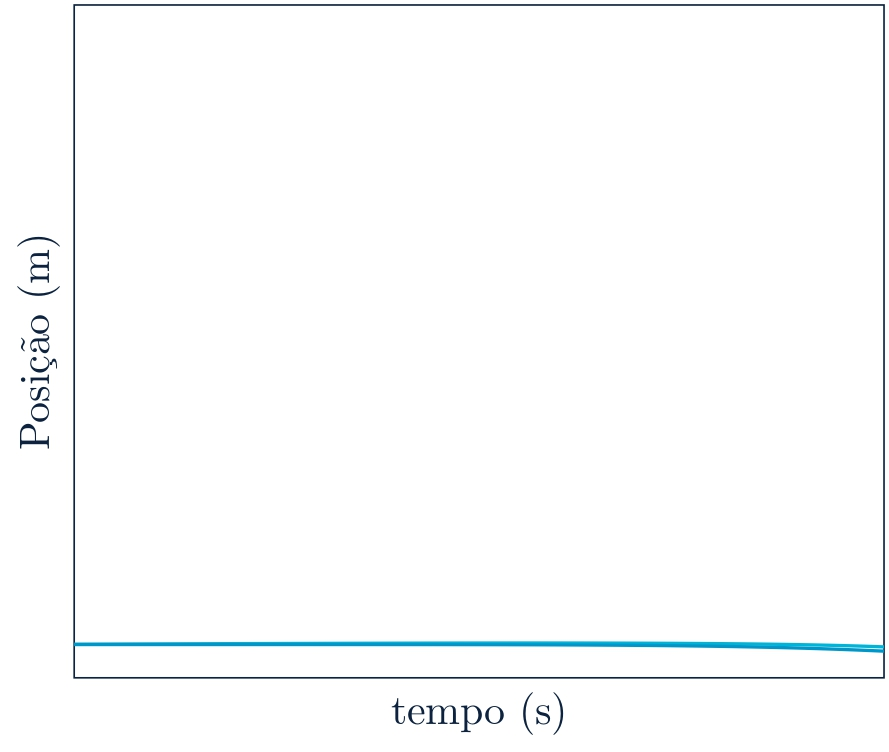
\includegraphics[width=0.3\columnwidth]{images/3.jpg}}
    \caption{(a) Resultados Bola 1 (b) Resultados Bola 2  (c) Resultados Bola 3}
    \label{fig:foobar}
\end{figure}

    Cras ut fermentum nunc, id interdum ex. Donec tincidunt metus nulla, a interdum ante efficitur cursus. Proin justo mauris, imperdiet vel efficitur ac, lobortis et neque. Etiam ac iaculis libero.

    \begin{table}
    \caption{Caption for table 1}
      \centering
      \begin{tabular}{c c c c }
        \toprule
        \textbf{Col 1} & \textbf{Col 2} & \textbf{Col 3} & \textbf{Col 4}\\
        \midrule
        A & 22 & 73 & 1.20\\
        B & 33.72 & 67 & 33.33\\
        C & 55.21 & 32 & 5.32\\
        {\color{blue}D} & 20 & 96.90 & {\color{blue}35.53}\\
        \bottomrule
      \end{tabular}
      \label{tab:table1}
\end{table}

\end{block}

% -------------------------------
% Section: Conclusions
% -------------------------------
   \begin{block}{Conclusões}
    \begin{itemize}
      \item Sed et augue accumsan nibh ullamcorper accumsanam dictum urna tortor, ut pretium leo eleifend.  
      \item Donec suscipit, urna quis tempus consectetur, quam est placerat ante, et scelerisque metus velit. 
      \item Nam dictum urna tortor, ut pretium leo eleifend efficitur.
      \item Praesent blandit faucibus quam, et tincidunt mauris sagittis eget 2.2\%.
      \item Dolor sit amet, consectetur adipiscing elit. Mauris in nulla ultricies suscipit.
    \end{itemize}
  \end{block}


% -------------------------------
% Section: What is already known about this subject?
% -------------------------------
  \begin{exampleblock}{What is already known about this subject?}

    \begin{itemize}
      \item \textbf{Lorem ipsum dolor sit amet}, consectetur adipiscing elit. Mauris in nulla ac leo ultricies suscipit.
      \item The \textbf{Duis vestibulum augue} in leo placerat, sit amet pharetra mi elementum.
      \item \textbf{Fusce sit amet} velit pulvinar, feugiat velit sit amet, tristique dolor.
    \end{itemize}

  \end{exampleblock}

  
% -------------------------------
% Section: What does this study add?
% -------------------------------
  \begin{exampleblock}{What does this study add?}
    \begin{itemize}
      \item Lorem ipsum dolor sit amet, consectetur adipiscing elit. Mauris in nulla ac leo ultricies suscipit.
      \item The Duis vestibulum augue in leo placerat, sit amet pharetra mi elementum.
      \item Fusce sit amet velit pulvinar, feugiat velit sit amet, tristique dolor.
    \end{itemize}

  \end{exampleblock}


% -------------------------------
% Section: Practical Implications
% -------------------------------
  \begin{exampleblock}{Practical implications}
    \begin{itemize}
      \item Ipsum dolor sit amet, consectetur adipiscing elit. Mauris in nulla ultricies suscipit.
      \item Duis augue in leo placerat, sit amet pharetra mi elementum.
      \item Sit amet pulvinar, feugiat velit sit amet, tristique dolor.
    \end{itemize}

  \end{exampleblock}

% -------------------------------
% Section: References
% ------------------------------- 

  \begin{block}{Referencias}

    \nocite{*}
    \footnotesize{\bibliographystyle{plainurl}\bibliography{poster}}

  \end{block}

% -------------------------------
% Section: Portfolio
% -------------------------------
  \begin{block}{Mais Informações}

    \begin{figure}[h]
    \centering
    
\includegraphics[height=8cm]{images/qrcode2.png}
    \label{fig:figure3}
\end{figure}

  \end{block}

\end{column}
\separatorcolumn



\end{columns}
\end{frame}

\end{document}
